%%
% 下のコメント欄は卒論執筆時の森がイキって書いたものです。
% 修論執筆時の森が代わりに謝罪いたします。
% 温かい目で見守ってあげてください。
%
% また、修論執筆時にはTeXstudioで、またDockerを用いて執筆しています。
% 上記の手法は平木場くんから教えていただきました。
% 参考: https://qiita.com/Shitimi_613/items/9706d57fb7bc17cbed0e
%

%%
% モダンなLaTeXを書きたい?
% そしたら僕の考えた最強のtexファイルを見てくれ
%
% 注意!
% このLaTeXをPDFに変換するためには、普通とはちょっと違う方法を使うよ
% コマンド上では
%   $ ptex2pdf -u -l GraduatePaper.tex
% で変換してね
% もしptex2pdfコマンドが無かったら、
%   $ uplatex GraduatePaper.tex
%   $ dvipdfmx GraduatePaper.dvi
% でうまくいくかも(未確認)
%
% え、TeXworksで使いたいって?
% そしたら、TeXworksの編集メニュー -> 設定を開く
% タイプセットタブの下の方にあるタイプセットの方法の右下の+ボタンを選択する
% 名前: uplatex(ptex2pdf)
% プログラム: ptex2pdf
% 引数: -l
%       -u
%       -ot
%       $synctexoption
%       $fullname
% として保存して、TeXworks実行ボタン右のコンボボックスのuplatex(ptex2pdf)を選択して変換だ!
%


%%
% 今時jarticleやjbook使ってる人いる?時代はjsarticleかjsbookだよ
% ついでに言うと、uplatexってのはplatexの上位互換、これを使わないなんて旧世代だよね
%
\documentclass[uplatex, report, a4j, 10pt, dvipdfmx]{jsbook}


%%
% パッケージ群
%
\usepackage{packages/miyazaki-u-paper}   % 宮崎大学工学部の卒論の基本(片山先生作)を、僕がちょっと書き換えちゃった(テヘッ
\usepackage{enumitem}           % enumerate?古い古い
\usepackage[dvipdfmx]{graphicx, color} % 当然dvipdfmなんて使ってないよね
% \usepackage[dvipdfmx]{color}    % listingsを使うときにはこれも必須、dvipdfmxを変えちゃうとgraphicxのdvipdfmxも変わるよ
\usepackage{listings, packages/jlisting} % コードを埋め込むなら必須
\usepackage{txfonts}            % フォントといえばやっぱりtxfonts、今はnewtxってのもあるらしい
\usepackage{verbatim}           % コメントアウトしてくれる便利なプリアンブルが使える \begin{comment} ... \end{comment}
\usepackage[hdivide={21mm, , 21mm}, vdivide={30mm, , 25mm}]{geometry} % スタイルを少し変えたくても\hoffset, \voffsetは使わないでね
%\RequirePackage[l2tabu, orthodox]{nag} % これを入れると、古いコマンドを警告してくれる!なお完全には消せなかった模様
%
% マクロの定義
%
\newcommand{\tool}{TOOL}
\newcommand{\toolFullName}{TOOL: Optimize Operation Language}

\renewcommand{\lstlistingname}{コード}
\lstset{
  language={Java},
  frame=tlBR,%フレーム線の指定,上右下左の順,大文字は二重線
%  frameround=tttt,%角の指定,右上|右下|左下|左上の順,tは丸角,fは四角
  framesep=5pt,%本文からframeまでの間隔
  framerule=.2pt,%線の太さ
%  rulecolor={\color[gray]},%線の色
%  backgroundcolor={\color[gray]{.9}},%背景色の指定
  basicstyle={\scriptsize\ttfamily \color[gray]{.15}},%書体の指定,この場合は7ptのタイプライタ体
  identifierstyle={\ttfamily},%識別子の書体
  keywordstyle={\ttfamily \color[cmyk]{0,1,0,0}},%言語ワードの書体
  stringstyle={\scriptsize\ttfamily \color[rgb]{0,0,1}},%文字列リテラルの書体
  commentstyle={\itshape \color[cmyk]{1,0,1,0}},%コメントの書体
  numberstyle={\scriptsize},%行番号の書式
  stepnumber=1,%行番号のステップ間隔
  numbers=left,%行番号の位置
  numbersep=1em,%本文との間隔
  breaklines=true,%改行の設定
  xleftmargin=0zw,
  xrightmargin=0zw,
  columns=[l]{fullflexible},
  lineskip=-0.5zw,
  morecomment={[s][{\color[cmyk]{1,0,0,0}}]{/**}{*/}},
  floatplacement=t,
  classoffset=1,
  showstringspaces=false,%空行の表示
%  breakatwhitespace=true,
%  tabsize=5,
}
\usepackage[dvipsnames]{xcolor}

% Kotlinのコードのハイライト
% 参考サイト
% https://github.com/cansik/kotlin-latex-listing
\lstdefinelanguage{Kotlin}{
  comment=[l]{//},
  commentstyle={\color{gray}\ttfamily},
  emph={delegate, filter, first, firstOrNull, forEach, lazy, map, mapNotNull, println, return@},
  emphstyle={\color{OrangeRed}},
  identifierstyle=\color{black},
  keywords={abstract, actual, as, as?, break, by, class, companion, continue, data, do, dynamic, else, enum, expect, false, final, for, fun, get, if, import, in, interface, internal, is, null, object, override, package, private, public, return, set, super, suspend, this, throw, true, try, typealias, val, var, vararg, when, where, while},
  keywordstyle={\color{NavyBlue}\bfseries},
  morecomment=[s]{/*}{*/},
  morestring=[b]",
  morestring=[s]{"""*}{*"""},
  ndkeywords={@Deprecated, @JvmField, @JvmName, @JvmOverloads, @JvmStatic, @JvmSynthetic, Array, Byte, Double, Float, Int, Integer, Iterable, Long, Runnable, Short, String},
  ndkeywordstyle={\color{BurntOrange}\bfseries},
  sensitive=true,
  stringstyle={\color{ForestGreen}\ttfamily},
}

% Swiftのコードのハイライト
% 参考サイト
% https://gist.github.com/chriseidhof/18dbc1c4eef919eab2c7
\lstdefinelanguage{swift}
{
  morekeywords={
    func,if,then,else,for,in,while,do,switch,case,default,where,break,continue,fallthrough,return,
    typealias,struct,class,enum,protocol,var,func,let,get,set,willSet,didSet,inout,init,deinit,extension,
    subscript,prefix,operator,infix,postfix,precedence,associativity,left,right,none,convenience,dynamic,
    final,lazy,mutating,nonmutating,optional,override,required,static,unowned,safe,weak,internal,
    private,public,is,as,self,unsafe,dynamicType,true,false,nil,Type,Protocol,
  },
  morecomment=[l]{//}, % l is for line comment
  morecomment=[s]{/*}{*/}, % s is for start and end delimiter
  morestring=[b]" % defines that strings are enclosed in double quotes
}

\definecolor{keyword}{HTML}{BA2CA3}
\definecolor{string}{HTML}{D12F1B}
\definecolor{comment}{HTML}{008400}

\lstset{
  language=swift,
  basicstyle=\ttfamily,
  showstringspaces=false, % lets spaces in strings appear as real spaces
  columns=fixed,
  keepspaces=true,
  keywordstyle=\color{keyword},
  stringstyle=\color{string},
  commentstyle=\color{comment},
}

%%
% miyazaki-u-paper.sty用設定値
%
\degree{m} % Graduateのg or Masterのm
\figurenumbering{f} % 図目次を付ける場合はt (真) を持つ真偽値を引数に取る関数
\tablenumbering{f} % 表目次を付ける場合はt (真) を持つ真偽値を引数に取る関数
\title{長ったらしいタイトルを \\ リアルタイムに描画するツール \\ \tool{}の実装と評価}
\author{執筆者ネーム}
\nendo{30} % 年度
\advisor{片山 徹郎 教授} % 修論では無視する
\major{工学専攻 機械・情報系コース 情報システム工学分野}



\begin{document}
\maketitle

\preface{概要}

ここには概要を書くよ


%%
% 本文
%
% はじめに
\chapter{はじめに}\label{cha:Introduction}

ここには初めにをかくほ

以下、本論文の構成は次のとおりである。

第\ref{cha:Preparation}章では、\tool{}を実装するために必要となる前提知識について説明する。

第\ref{cha:Appearance}章では、\tool{}の外観について説明する。

第\ref{cha:Function}章では、\tool{}の機能について説明する。

第\ref{cha:Implementation}章では、\tool{}の実装について説明する。

第\ref{cha:Indication}章では、試作した\tool{}を用いてUMLとソースコードを記述し、\tool{}が正しく動作することを検証する。

第\ref{cha:Evaluation}章では、\tool{}について考察する。

第\ref{cha:Conclusion}章では、本研究のまとめと今後の課題を示す。



% 研究の準備
\chapter{研究の準備}\label{cha:Preparation}

本章では、\tool{}を実装するにあたり、必要となる前提知識を説明する。
\section{Kotlinの参考コード}

\begin{lstlisting}[caption={Kotlinの参考コード}, label={lst:example1}, language=Kotlin]
// this is a simple code listing:
println("Hello, World")
\end{lstlisting}

\section{Swiftの参考コード}

\begin{lstlisting}[caption={Swiftの参考コード}, label={lst:example2}, language=swift]
// this is a simple code listing:
@IBAction func backButton(_ sender: Any) {
  performSegue(withIdentifier: "toViewController", sender: nil)
}
\end{lstlisting}



% 外観
\chapter{\tool{}の外観}\label{cha:Appearance}

本章では、本研究で実装したツール\tool{} (\toolFullName{})の外観について説明する。

\tool{}の外観を、図hogehogeに示す。


% 機能
\chapter{\tool{}の機能}\label{cha:Function}

本章では、\tool{}の機能について説明する。
\tool{}は、大きく分けて以下の3つの機能を持つ。

\begin{itemize}
	\item 機能1
	\item 機能2
	\item 機能3
\end{itemize}

以降、各機能について説明する。



\section{機能1}

\section{機能2}
\section{機能3}

% 実装
\chapter{\tool{}の実装}\label{cha:Implementation}

本章では、\tool{}の実装について説明する。
\tool{}の構造とデータ遷移を、図\ref{fig:toolStructure}に示す。

\begin{figure}[t]
	\centering
	
\includegraphics[width=.8\linewidth]{./figs/breadboard.eps}
	\caption{\tool{}の構造とデータ遷移}
	\label{fig:toolStructure}
\end{figure}

\begin{figure}[tp]
  \begin{center}
  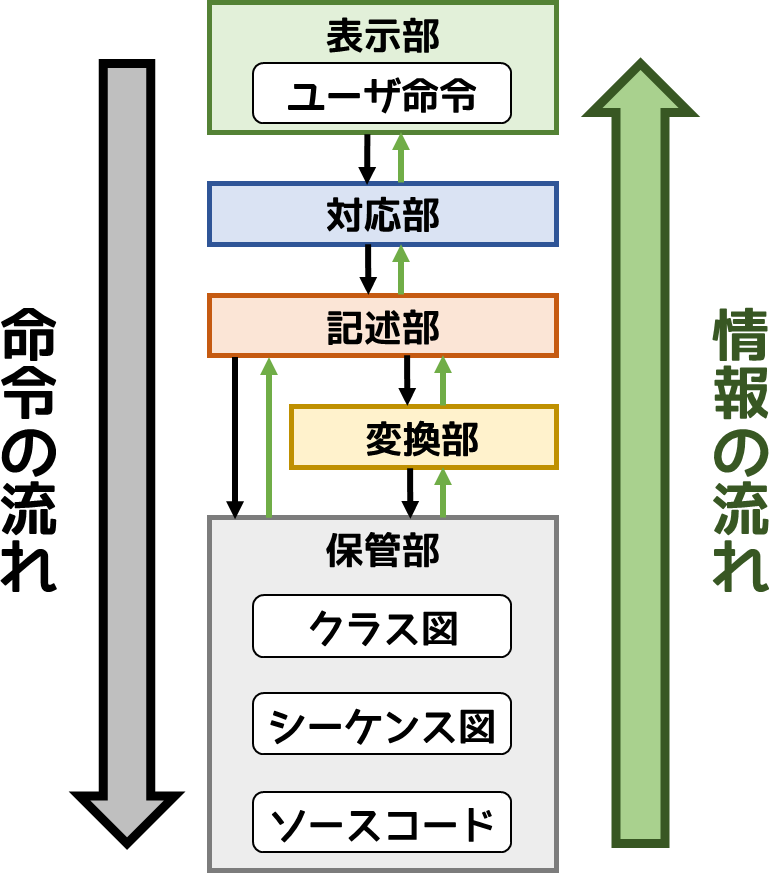
\includegraphics[width=160mm]{./figs/retussStructure.png}
	\caption{\tool{}の構造とデータ遷移}
	\label{fig:toolStructure2}
\end{center}
\end{figure}

% 適用例
\chapter{適用例}\label{cha:Indication}

% 考察
\chapter{考察}\label{cha:Evaluation}

% おわりに
\chapter{おわりに} \label{cha:Conclusion}

%%
% 謝辞
%
\acknowledgment{}

謝辞をかくよ


%%
% 参考文献
%
\begin{thebibliography}{99}
  % 森氏の成果物
  \bibitem{ICAROB2019} Keisuke Mori, Tetsuro Katayama, Yoshihiro Kita, Hisaaki Yamaba, Kentaro Aburada, and Naonobu Okazaki: ``Development of Library Fescue Extracting Elements of Attributes and Operations of Class Diagram in UML,'' The 2019 International Conference on Artificial Life and Robotics (ICAROB2019), pp. 165--168, 2019
  
  \bibitem{Fescue} GitHub: ``Fescue: Feature Elements Section of Class in UML Extraction,'' https://github.com/Morichan/Fescue (最終アクセス 2019/01/25)
  \end{thebibliography}

%%
% 付録
%
% \appendix{} % 付録は基本的に使わない

\end{document}
